\documentclass[tikz,border=8pt]{standalone}
% Style commun des schémas : thème clair / sombre (couleurs des thèmes GitHub), fond transparent.
\usepackage[T1]{fontenc}
\usepackage{tgheros}
\renewcommand{\familydefault}{\sfdefault}
\usepackage{tikz}
\usetikzlibrary{positioning,arrows.meta,calc,fit,backgrounds}
\ifdefined\darktheme
  \definecolor{fg}{HTML}{E6EDF3}  \definecolor{muted}{HTML}{9198A1}
  \definecolor{line}{HTML}{8B949E} \definecolor{boxfill}{HTML}{151B23}
  \definecolor{boxline}{HTML}{3D444D}
  \definecolor{blue}{HTML}{4493F8} \definecolor{orange}{HTML}{DB6D28}
  \definecolor{green}{HTML}{3FB950} \definecolor{red}{HTML}{F85149}
  \definecolor{purple}{HTML}{AB7DF8}
\else
  \definecolor{fg}{HTML}{1F2328}  \definecolor{muted}{HTML}{59636E}
  \definecolor{line}{HTML}{59636E} \definecolor{boxfill}{HTML}{F6F8FA}
  \definecolor{boxline}{HTML}{D1D9E0}
  \definecolor{blue}{HTML}{0969DA} \definecolor{orange}{HTML}{BC4C00}
  \definecolor{green}{HTML}{1A7F37} \definecolor{red}{HTML}{CF222E}
  \definecolor{purple}{HTML}{8250DF}
\fi
\tikzset{
  every node/.style={text=fg, font=\small},
  block/.style={draw=boxline, fill=boxfill, rounded corners=3pt, line width=0.7pt,
                minimum height=11mm, minimum width=30mm, align=center, inner sep=5pt},
  sub/.style={font=\scriptsize, text=muted},
  wire/.style={line width=1pt, -{Stealth[length=2.6mm]}},
  biwire/.style={line width=1pt, {Stealth[length=2.6mm]}-{Stealth[length=2.6mm]}},
  lbl/.style={font=\scriptsize, text=muted, fill=none, inner sep=2pt},
}

\definecolor{mk}{HTML}{111111}\definecolor{mw}{HTML}{F5F5F5}
\begin{document}
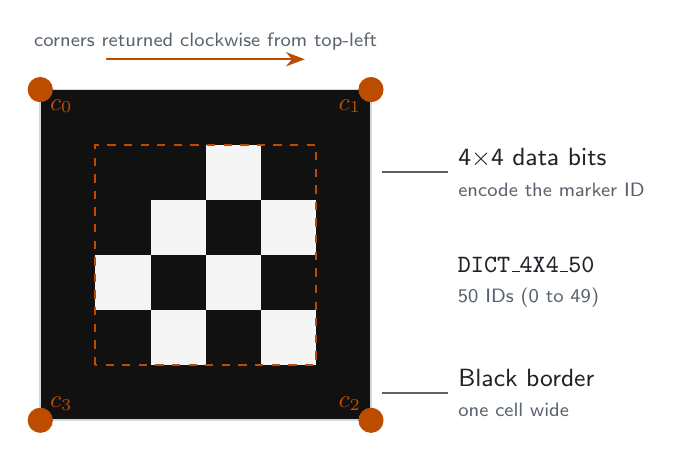
\begin{tikzpicture}[x=7mm,y=7mm]
  % marqueur 6x6 : bordure noire d'une case + 4x4 bits de données (exemple)
  \fill[mk] (0,0) rectangle (6,6);
  \foreach \r/\row in {0/{1,1,0,1}, 1/{1,0,1,0}, 2/{0,1,0,1}, 3/{1,0,1,0}}{
    \foreach \b [count=\c from 0] in \row {
      \ifnum\b=0 \fill[mw] (\c+1,4-\r) rectangle ++(1,1); \fi
    }
  }
  \draw[boxline, line width=0.6pt] (0,0) rectangle (6,6);
  \draw[orange, dashed, line width=0.8pt] (1,1) rectangle (5,5);
  % coins dans l'ordre d'OpenCV
  \foreach \p/\n/\a in {(0,6)/c_0/north west, (6,6)/c_1/north east, (6,0)/c_2/south east, (0,0)/c_3/south west}{
    \fill[orange] \p circle (1.6mm);
    \node[anchor=\a, text=orange, font=\small] at \p {$\n$};
  }
  \draw[orange, -{Stealth[length=2.4mm]}, line width=0.8pt] (1.2,6.55) -- (4.8,6.55);
  \node[lbl, above] at (3,6.6) {corners returned clockwise from top-left};
  % annotations
  \draw[line, line width=0.7pt] (6.2,4.5) -- (7.4,4.5) node[right, align=left, font=\small]{4$\times$4 data bits\\\textcolor{muted}{\scriptsize encode the marker ID}};
  \draw[line, line width=0.7pt] (6.2,0.5) -- (7.4,0.5) node[right, align=left, font=\small]{Black border\\\textcolor{muted}{\scriptsize one cell wide}};
  \node[right, align=left, font=\small] at (7.4,2.5) {\texttt{DICT\_4X4\_50}\\\textcolor{muted}{\scriptsize 50 IDs (0 to 49)}};
\end{tikzpicture}
\end{document}
